\documentclass[a4paper,11pt]{uos-thesis}

% ******************************* Thesis Glossary ***************************
\setabbreviationstyle[acronym]{long-short}

\newacronym{bilp}{BILP}{Binary Integer Linear Programming}
\newacronym{bmi}{BMI}{Bilinear Matrix Inequality}
\newacronym{cp}{CP}{Cone Programming}
\newacronym{eec}{EEC}{Electronic Engine Controller}
\newacronym{epr}{EPR}{Engine Pressure Ratio}
\newacronym{fadec}{FADEC}{Full Authority Digital Engine Controller}
\newacronym{flops}{FLOPS}{Floating Point Operations Per Second}
\newacronym{gp}{GP}{Geometric Programming}
\newacronym{gte}{GTE}{Gas Turbine Engine}
\newacronym{ilp}{ILP}{Integer Linear Programming}
\newacronym[longplural={Linear Matrix Inequalities}]{lmi}{LMI}{Linear Matrix Inequality}
\newacronym{lp}{LP}{Linear Programming}
\newacronym{lpv}{LPV}{Linear Parameter-varying}
\newacronym{lqr}{LQR}{Linear Quadratic Regulator}
\newacronym{lti}{LTI}{Linear Time-invariant}
\newacronym{milp}{MILP}{Mixed Integer Linear Programming}
\newacronym{mpc}{MPC}{Model Predictive Control}
\newacronym{np}{NP}{Non-deterministic Polynomial}
\newacronym{p}{P}{Polynomial Deterministic}
\newacronym{pid}{PID}{Proportional Derivative Integral}
\newacronym{qcqp}{QCQP}{Quadratic Constraint Quadratic Programm\-ing}
\newacronym{qp}{QP}{Quadratic Programming}
\newacronym{sdp}{SDP}{Semi-definite Programming}
\newacronym{socp}{SOCP}{Second-order Cone Programming}
 % Glossary

\begin{document}

\frontmatter
% ************************** Thesis Title*****************************
\begin{titlepage}

\begin{flushleft}
\includegraphics[width=0.5\textwidth]{Title/Figures/UoSLogo}
\end{flushleft}

\vspace*{1cm}

\Huge{\textbf{Thesis title}}
        
\vspace{0.5cm}
        \Large Research group name
        \\
        \large Author: Author name
        \vspace{2.5cm}
        
        \LARGE PhD Thesis\\
        \small A dissertation submitted for the degree of\\
        Doctor of Philosophy
        \vspace{2cm}

        \normalsize
        Department of Automatic Control \& Systems Engineering\\
        University of Sheffield\\
        United Kingdom\\
        \today

\end{titlepage}
\include{Declaration/declaration}
% ******************************* Thesis Quote ***************************
\thispagestyle{empty}  % No headers or footers for the following pages
\null\vfill

% Quote written in italics
\textit{``Imagination is more important than knowledge''}

\begin{flushright}
Albert Einstein
\end{flushright}

\vfill\vfill\vfill\vfill\vfill\vfill\null
% ******************************* Thesis Abstract ***************************
\chapter{Abstract}

This is my latex thesis template

\blfootnote{\textbf{Keywords: my list of keywords}}
% ******************************* Thesis Acknowledgements ***************************
\chapter{Acknowledgements}

First of all, I would like to give a special thanks to my supervisory team, especially XXX for his valuable support and guidance throughout my research as well as for his general availability.
\bigbreak
Some other acknowledgements
\bigbreak
Some different acknowledgments...
\bigbreak
Last but not least, the last acknowledgements !
% ******************************* Thesis Nomenclature ***************************

% Scalar Sets
\nomenclature[A00]{$\mathbb{N}$}{Set of natural numbers}
\nomenclature[A01]{$\mathbb{N}^{*}$}{Set of natural numbers, zero excluded}
\nomenclature[A02]{$\llbracket a,b \rrbracket$}{Set of integers $\{a,\ldots , b \}$}
\nomenclature[A03]{$\mathbb{Z}$}{Set of integers}
\nomenclature[A04]{$\mathbb{R}$}{Set of real numbers}
\nomenclature[A05]{$\mathbb{R}^{*}$}{Set of real numbers, zero excluded}
\nomenclature[A06]{$\mathbb{R}_{+}$}{Set of positive real numbers}
\nomenclature[A07]{$\mathbb{R}_{+}^{*}$}{Set of strictly positive real numbers}
\nomenclature[A08]{$\mathbb{C}$}{Set of complex numbers}
\nomenclature[A09]{$\mathbb{C}_{+}$}{Set of complex numbers with positive real part}
\nomenclature[A10]{$\mathbb{C}_{+}^{*}$}{Set of complex numbers with strictly positive real part}
\nomenclature[A11]{$\mathbb{R}^{n}$}{Set of real vectors of dimension $n$}
\nomenclature[A12]{$ \mathbb{R}^{n \times m} $}{Set of real matrices of dimension ${n \times m}$}
\nomenclature[A13]{$ \mathbb{S}^{n}$}{Set of symmetric matrices of dimension ${n}$}
\nomenclature[A14]{$ \mathbb{S}^{n}_{+}$}{Set of symmetric positive semi-definite matrices of dimension ${n}$}
\nomenclature[A15]{$ \mathbb{S}^{n}_{++}$}{Set of symmetric positive definite matrices of dimension ${n}$}

% Generalized Inequalities
\nomenclature[B00]{$x \geq y$}{Element-wise inequality between $x$ and $y$}
\nomenclature[B01]{$x > y$}{Strict element-wise inequality between $x$ and $y$}
\nomenclature[B02]{$X \succeq 0$}{$X$ is positive semi-definite: ${X \in \mathbb{S}^{n}_{+}}$}
\nomenclature[B03]{$X \succ 0$}{$X$ is positive definite: ${X \in \mathbb{S}^{n}_{++}}$}
\nomenclature[B04]{$X \succeq Y$}{Matrix inequality between symmetric matrices: \\ ${(X-Y) \in \mathbb{S}^{n}_{+}}$}
\nomenclature[B05]{$X \succ Y$}{Strict matrix inequality between symmetric matrices: \\ ${(X-Y) \in \mathbb{S}^{n}_{++}}$}
\nomenclature[B06]{$X \succeq_{K} Y$}{Conic inequality between $X$ and $Y$: \\ ${(X-Y) \in K}$}
\nomenclature[B07]{$X \succ_{K} Y$}{Strict conic inequality between $X$ and $Y$: \\ ${(X-Y) \in \operatorname{int}K}$}

% Norms
\nomenclature[C00]{$\lvert z \rvert$}{The magnitude of a complex number $z$}
\nomenclature[C01]{$\lVert x \rVert_{0}$}{$l_{0}$-norm operator applied to the vector $x$}
\nomenclature[C02]{$\lVert x \rVert_{1}$}{$l_{1}$-norm operator applied to the vector $x$}
\nomenclature[C03]{$\lVert x \rVert_{2}$}{$l_{2}$-norm operator applied to the vector $x$}
\nomenclature[C04]{$\lVert x \rVert_{Q}$}{$Q$-weighted $l_{2}$-norm operator applied to the vector $x$}
\nomenclature[C05]{$\lVert x \rVert_{\infty}$}{$l_{\infty}$-norm operator applied to the vector $x$}
\nomenclature[C06]{$\lVert X \rVert_{2}$}{Spectral norm operator applied to the matrix $X$}

% Vectors & Matrices
\nomenclature[D00]{$e_{i}$}{${i^{th}}$ canonical unit vector of appropriate dimension}
\nomenclature[D01]{$I_{n}$}{Identity matrix in ${\mathbb{R}^{n \times n}}$}
\nomenclature[D02]{$0_{n \times m}$}{Zero matrix of dimension ${n \times m}$, used without subscripts}
\nomenclature[D03]{$A^{\top}$}{Transpose of the matrix $A$}
\nomenclature[D04]{$\operatorname{rank}(A)$}{Rank of the matrix $A$}
\nomenclature[D05]{$\operatorname{tr}(A)$}{Trace of the matrix $A$}
\nomenclature[D06]{$\operatorname{vec}(A)$}{Vectorization of the matrix $A$}
\nomenclature[D07]{$\lambda_{max}(A), \lambda_{min}(A)$}{Maximum, minimum eigenvalue of the matrix $A$}
\nomenclature[D08]{$\sigma_{max}(A), \sigma_{min}(A)$}{Maximum, minimum singular value of the matrix $A$}
\nomenclature[D09]{$\lvert A \rvert$}{The magnitude operator is applied to each element of $A$}
\nomenclature[D10]{$A \circ B$}{Hadamard product of two matrices $A$ and $B$}
\nomenclature[D11]{$[A \vert B]$}{Horizontal concatenation of the matrices $A$ and $B$}

% Set Operations
\nomenclature[E00]{$S_{1} \cup S_{2}$}{Union of sets $S_{1}$ and $S_{2}$}
\nomenclature[E01]{$S_{1} \cap S_{2}$}{Intersection of sets $S_{1}$ and $S_{2}$}
\nomenclature[E02]{$S_{1} \times S_{2}$}{Cartesian product of sets $S_{1}$ and $S_{2}$}
\nomenclature[E03]{$S_{1} \oplus S_{2}$}{Minkowski sum of sets $S_{1}$ and $S_{2}$}
\nomenclature[E04]{$S_{1} \ominus S_{2}$}{Pontryagin difference of sets $S_{1}$ and $S_{2}$}


\tableofcontents
\listoffigures
\listoftables
\printglossary
\printnomenclature
% ******************************* Thesis Latin Quote ***************************
\thispagestyle{empty}  % No headers or footers for the following pages
\null\vfill

% Quote written in italics
\textit{``D\={\i}vide et imper\={a}''}

\begin{flushright}
Philip of Macedonia
\end{flushright}

\vfill\vfill\vfill\vfill\vfill\vfill\null

\mainmatter
%*******************************************************************************
%*********************************** First Chapter *****************************
%*******************************************************************************
\chapter{Introduction} 
\chaptermark{Introduction}
\label{Chap1}

Introduction, this is my first chapter. This thesis is written in \LaTeX\ based on the following resource \citep{Lamport1985}

\begin{figure}[htbp]
\centering

\includegraphics[scale=1]{Chapters/Chapter1/LaTeX_cover}
\caption{Vectorial picture example.}
\label{fig1}
\end{figure}

The Figure \eqref{fig1} comes from the following source: \url{https://en.wikibooks.org/wiki/LaTeX}

\section{First Section}

This is my first section of the first chapter
\blindtext[2]

\subsection{First subsection}

This is my first subsection of the first section of the first chapter
\blindtext[2] % Introduction
%*******************************************************************************
%********************************* Second Chapter ****************************
%*******************************************************************************
\chapter{Chapter Two}
\chaptermark{Chapter 2}
\label{Chap2}

\section{Introduction}

This is the introduction of my second chapter with the use of some acronym like \gls{lti} (first use in a chapter). The second use of the acronym \gls{lti} is different.
 % Chapter 2
%*******************************************************************************
%*********************************** Third Chapter *****************************
%*******************************************************************************
\chapter{Chapter Three}
\chaptermark{Chapter 3}
\label{Chap3}

\section{Introduction}

\blindtext[5]

\section{Some mathematical section}

\begin{theorem}
The Pythagoras theorem can be stated as follows,
\begin{equation}
a^{2} + b^2 = c^{2}, 
\end{equation}
where $c$ represents the hypotenuse of a rectangle triangle and $a$ and $b$ represent the other sides.
\end{theorem}

\begin{proof}
The proof is given by Pythagoras in the documents here.
\end{proof} % Chapter 3
%\include{Chapters/Chapter4/chapter4} % To include chapter 4 create a Tex file
% The thesis can be compiled with only a subsection of the chapters

\appendix
%*******************************************************************************
%********************************* Appendix A **********************************
%*******************************************************************************
\chapter{Appendix A}
\chaptermark{Appendix A}
\label{AppendixA}

\section{Introduction}

Number theory is a field of mathematics that studies integers, it subsumes the branch of combinatorics concerned with counting the number of combinations and permutations of finite sets \citep{Laplace1820}. The Stirling numbers of first, second and third kind play an important role in combinatorial mathematics, they find applications for different analytic and combinatorial problems and they can all be used to express the coefficient of sequences of polynomials. All these numbers are linked by the fact that they can express the number of partitions of a set with $n$ elements into $k$ non-empty non-overlapping subsets. This appendix aims at introducing the Stirling numbers as well as how they can be computed. Also, a presentation of some of their properties as well as the link between them is also provided.

\section{Stirling Numbers of the First Kind}

The Stirling numbers of the first kind are linked to the number of cycles within a finite discrete set. These numbers can be unsigned or signed and are defined by the coefficients of the rising and falling factorials as follows,

\begin{equation} \label{eqnA.1}
x^{(n)} = \prod_{k=0}^{n-1} (x+k) = \sum_{k=0}^{n} \genfrac{[}{]}{0pt}{0}{n}{k} x^{k}.
\end{equation}

The equation \eqref{eqnA.1} defines the rising factorial and its relation with the unsigned Stirling numbers of the first kind, whereas the equation \eqref{eqnA.2} defines the falling factorial along with its relation with the unsigned Stirling numbers of the first kind. The signed Stirling numbers of the first kind are obtained by combining the sign in the sum of \eqref{eqnA.2} with the unsigned Stirling numbers of the first kind.

\begin{equation} \label{eqnA.2}
(x)_{n} = \prod_{k=0}^{n-1} (x-k) = \sum_{k=0}^{n} (-1)^{n-k} \genfrac{[}{]}{0pt}{0}{n}{k} x^{k} 
\end{equation}

The unsigned Stirling numbers of the first kind correspond to the number of permutations of a set of $n$ elements with $k$ disjoint cycles. These numbers can also be computed using the following recurrence relation,

\begin{subequations} \label{eqnA.3}
\begin{align}
\forall (n,k) \in \mathbb{N}^{*} \times \mathbb{N}^{*} ,\, & \genfrac{[}{]}{0pt}{0}{0}{0} = 1 ,\, \genfrac{[}{]}{0pt}{0}{n}{0} = \genfrac{[}{]}{0pt}{0}{0}{n} = 0, \label{eqnA.3a} \\
& \genfrac{[}{]}{0pt}{0}{n+1}{k} = \genfrac{[}{]}{0pt}{0}{n}{k-1} + n \genfrac{[}{]}{0pt}{0}{n}{k}. \label{eqnA.3b}
\end{align}
\end{subequations}

It is possible to show this recurrence relation using either the definition of the Stirling numbers of first kind based on the rising or falling factorials or by using their combinatorial definition based on permutations. The first few Stirling numbers of the first kind are presented within Table \ref{tabA.1}.

\begin{table}[!htbp]
\centering
\caption{Stirling numbers of the first kind.}
\label{tabA.1}
\begin{tabular}{ccccccc}
\toprule
$n \backslash k$ & 0 & 1 & 2 & 3 & 4 & 5 \\
\cmidrule(lr){1-7}
0 & 1 & & & & & \\
1 & 0 & 1 & & & & \\
2 & 0 & 1 & 1 & & & \\
3 & 0 & 2 & 3 & 1 & & \\
4 & 0 & 6 & 11 & 6 & 1 & \\
5 & 0 & 24 & 50 & 35 & 10 & 1 \\
\bottomrule
\end{tabular}
\end{table}

For a fixed value of $n$, the sum of all the Stirling numbers of the first kind over $k$ from $0$ to $n$ yields factorial $n$, which can be computed from the rising factorial with $x$ equal $1$.

\begin{equation} \label{eqnA.4}
\forall n \in \mathbb{N} ,\, \sum_{k=0}^{n} \genfrac{[}{]}{0pt}{0}{n}{k} = n! = \genfrac{[}{]}{0pt}{0}{n+1}{1}
\end{equation}

Using the recursive relation \eqref{eqnA.3}, it is trivial to show that the right side equality of \eqref{eqnA.4} holds.

\begin{figure}[!htbp]
\centering
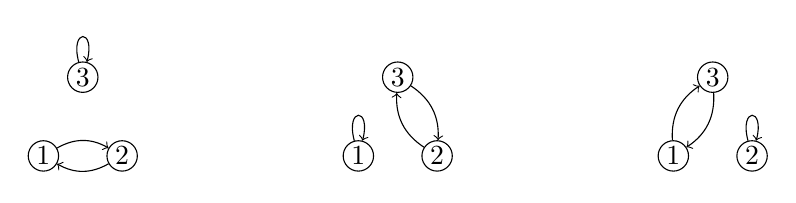
\begin{tikzpicture}
% Set left
\draw (-4,+0) node(n11)[circle,draw=black,inner sep=1pt] {$1$} +(1,0) node(n12)[circle,draw=black,inner sep=1pt] {$2$} +(0.5,1) node(n13)[circle,draw=black,inner sep=1pt] {$3$};
% Set middle
\draw (+0,+0) node(n21)[circle,draw=black,inner sep=1pt] {$1$} +(1,0) node(n22)[circle,draw=black,inner sep=1pt] {$2$} +(0.5,1) node(n23)[circle,draw=black,inner sep=1pt] {$3$};
% Set right
\draw (+4,+0) node(n31)[circle,draw=black,inner sep=1pt] {$1$} +(1,0) node(n32)[circle,draw=black,inner sep=1pt] {$2$} +(0.5,1) node(n33)[circle,draw=black,inner sep=1pt] {$3$};
% Arrows set 1
\draw[->] (n11) edge [bend left] (n12);
\draw[->] (n12) edge [bend left] (n11);
\draw[->] (n13) edge [loop,out=105,in=75,looseness=11] (n13);
% Arrows set 2
\draw[->] (n22) edge [bend left] (n23);
\draw[->] (n23) edge [bend left] (n22);
\draw[->] (n21) edge [loop,out=105,in=75,looseness=11] (n21);
% Arrows set 3
\draw[->] (n33) edge [bend left] (n31);
\draw[->] (n31) edge [bend left] (n33);
\draw[->] (n32) edge [loop,out=105,in=75,looseness=11] (n32);
\end{tikzpicture}
\caption{Cycle representations of the Stirling number of the first kind with $n=3$ and $k=2$.}
\label{figA.1}
\end{figure}

Figure \ref{figA.1} represents the different cycles linked to the Stirling number of the first kind with a set of $n=3$ elements and $k=2$ cycles. The total number of ways to partition the set is $3$. In this case, all three partitions have a cycle composed of $2$ elements and a cycle of a single element.

\section{Stirling Numbers of the Second Kind}

The Stirling numbers of the second kind represent the number of ways to partition a set of $n$ elements into $k$ non-empty non-overlapping subsets. These numbers are the inverse to the Stirling numbers of the first kind. Similarly to the Stirling number of the first kind, they can be computed based on the generating function consisting of the rising and falling factorials \eqref{eqnA.5}, such that,

\begin{equation} \label{eqnA.5}
\forall n \in \mathbb{N} ,\, x^{n} = \sum_{k=0}^{n} \genfrac{\{}{\}}{0pt}{0}{n}{k} (x)_{k} = \sum_{k=0}^{n} (-1)^{n-k}\genfrac{\{}{\}}{0pt}{0}{n}{k} x^{(k)}
\end{equation}

It can be proved that there exists a recurrence relation between the Stirling number of the second kind based on their definition from the falling factorial. The recurrence relation is as follows,

\begin{subequations} \label{eqnA.6}
\begin{align}
\forall (n,k) \in \mathbb{N}^{*} \times \mathbb{N}^{*} ,\, & \genfrac{\{}{\}}{0pt}{0}{0}{0} = 1 ,\, \genfrac{\{}{\}}{0pt}{0}{n}{0} = \genfrac{\{}{\}}{0pt}{0}{0}{n} = 0, \label{eqnA.6a} \\
& \genfrac{\{}{\}}{0pt}{0}{n+1}{k} = k \genfrac{\{}{\}}{0pt}{0}{n}{k} + \genfrac{\{}{\}}{0pt}{0}{n}{k-1}. \label{eqnA.6b}
\end{align}
\end{subequations}

Table \ref{tabA.2} presents the first few Stirling numbers of the second kind which highlights the recurrence relation presented previously.

\begin{table}[!htbp]
\centering
\caption{Stirling numbers of the second kind.}
\label{tabA.2}
\begin{tabular}{ccccccc}
\toprule
$n \backslash k$ & 0 & 1 & 2 & 3 & 4 & 5 \\
\cmidrule(lr){1-7}
0 & 1 & & & & & \\
1 & 0 & 1 & & & & \\
2 & 0 & 1 & 1 & & & \\
3 & 0 & 1 & 3 & 1 & & \\
4 & 0 & 1 & 7 & 6 & 1 & \\
5 & 0 & 1 & 15 & 25 & 10 & 1 \\
\bottomrule
\end{tabular}
\end{table}

There is an explicit formula used to compute the Stirling numbers of the second kind relying on factorials, this formula is as follows,

\begin{equation} \label{eqnA.7}
\genfrac{\{}{\}}{0pt}{0}{n}{k} = \frac{1}{k!} \sum_{i=0}^{k} (-1)^{k-i} \genfrac{(}{)}{0pt}{0}{k}{i} i^{n}.
\end{equation}

The total number of ways to partition a set with $n$ elements into non-empty non-overlapping subsets is defined by the Bell number. Consequently, the $n$-th Bell number $B_{n}$ is equal to the sum of the Stirling numbers of the second kind such that,

\begin{equation} \label{eqnA.8}
\forall n \in \mathbb{N} ,\, \sum_{k=0}^{n} \genfrac{\{}{\}}{0pt}{0}{n}{k} = B_{n}.
\end{equation}

In order to have an idea of the distinct ways to partition a set of $n$ elements into $k$ non-empty non-overlapping subsets, the Figure \ref{figA.2} illustrates all the different partitioning ways with $n=4$ and $k=2$. In this case, there are $6$ possible ways the partition the set of four elements, each one is composed of a subset composed of two elements as well as two subsets with a single element.

\begin{figure}[!htbp]
\centering
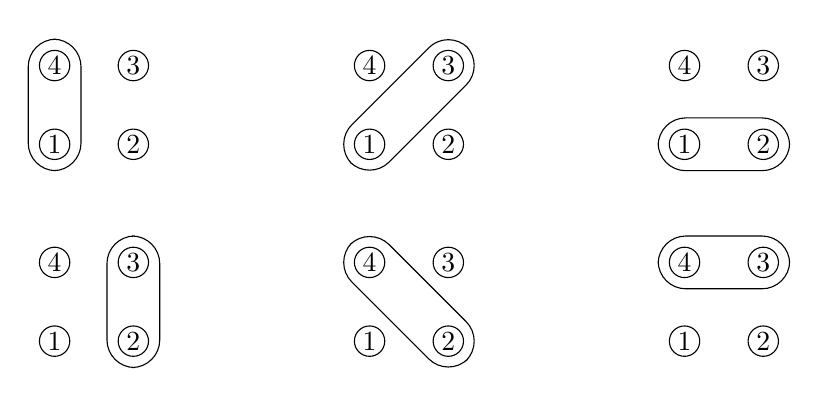
\begin{tikzpicture}[every node/.style={outer sep=8pt}]
% Set top left
\draw (-4,+2.5) node(n11)[circle,draw=black,inner sep=1pt] {$1$} +(1,0) node(n12)[circle,draw=black,inner sep=1pt] {$2$} +(1,1) node(n13)[circle,draw=black,inner sep=1pt] {$3$} +(0,1) node(n14)[circle,draw=black,inner sep=1pt] {$4$};
% Set top middle
\draw (+0,+2.5) node(n21)[circle,draw=black,inner sep=1pt] {$1$} +(1,0) node(n22)[circle,draw=black,inner sep=1pt] {$2$} +(1,1) node(n23)[circle,draw=black,inner sep=1pt] {$3$} +(0,1) node(n24)[circle,draw=black,inner sep=1pt] {$4$};
% Set top right
\draw (+4,+2.5) node(n31)[circle,draw=black,inner sep=1pt] {$1$} +(1,0) node(n32)[circle,draw=black,inner sep=1pt] {$2$} +(1,1) node(n33)[circle,draw=black,inner sep=1pt] {$3$} +(0,1) node(n34)[circle,draw=black,inner sep=1pt] {$4$};
% Set bottom left
\draw (-4,+0) node(n41)[circle,draw=black,inner sep=1pt] {$1$} +(1,0) node(n42)[circle,draw=black,inner sep=1pt] {$2$} +(1,1) node(n43)[circle,draw=black,inner sep=1pt] {$3$} +(0,1) node(n44)[circle,draw=black,inner sep=1pt] {$4$};
% Set bottom middle
\draw (+0,+0) node(n51)[circle,draw=black,inner sep=1pt] {$1$} +(1,0) node(n52)[circle,draw=black,inner sep=1pt] {$2$} +(1,1) node(n53)[circle,draw=black,inner sep=1pt] {$3$} +(0,1) node(n54)[circle,draw=black,inner sep=1pt] {$4$};
% Set bottom right
\draw (+4,+0) node(n61)[circle,draw=black,inner sep=1pt] {$1$} +(1,0) node(n62)[circle,draw=black,inner sep=1pt] {$2$} +(1,1) node(n63)[circle,draw=black,inner sep=1pt] {$3$} +(0,1) node(n64)[circle,draw=black,inner sep=1pt] {$4$};
% Subsets
\path[draw=black,rounded corners=10pt] (n11.south east) -- (n14.north east) -- (n14.north west) -- (n11.south west) -- cycle;
\path[draw=black,rounded corners=10pt] (n21.south) -- (n23.east) -- (n23.north) -- (n21.west) -- cycle;
\path[draw=black,rounded corners=10pt] (n31.south west) -- (n32.south east) -- (n32.north east) -- (n31.north west) -- cycle;
\path[draw=black,rounded corners=10pt] (n42.south east) -- (n43.north east) -- (n43.north west) -- (n42.south west) -- cycle;
\path[draw=black,rounded corners=10pt] (n52.east) -- (n54.north) -- (n54.west) -- (n52.south) -- cycle;
\path[draw=black,rounded corners=10pt] (n64.south west) -- (n63.south east) -- (n63.north east) -- (n64.north west) -- cycle;
\end{tikzpicture}
\caption{Set partitions representing the Stirling number of the second kind with $n=4$ and $k=3$.}
\label{figA.2}
\end{figure}

\section{Lah Numbers}

The Lah numbers, also sometimes called the Stirling numbers of the third kind, represent the number of ways to partition a set of $n$ elements into $k$ non-empty non-overlapping ordered subsets. Similarly to the Stirling number of the first and second kinds, the Lah numbers can be generated using the rising factorial as follows,

\begin{equation} \label{eqnA.9}
x^{(n)} = \sum_{k=1}^{n} \genfrac{\lfloor}{\rfloor}{0pt}{0}{n}{k} (x)_{k}.
\end{equation}

In the same fashion as for the Stirling numbers of the first and second kinds, the Lah numbers are linked to the falling factorial, the relation is as follows,

\begin{equation} \label{eqnA.10}
(x)_{n} = \sum_{k=1}^{n} (-1)^{n-k} \genfrac{\lfloor}{\rfloor}{0pt}{0}{n}{k} x^{(k)}.
\end{equation}

The Lah numbers can be calculated by using the following recurrence relation,

\begin{subequations} \label{eqnA.11}
\begin{align}
\forall (n,k) \in \mathbb{N}^{*} \times \mathbb{N}^{*} ,\, & \genfrac{\lfloor}{\rfloor}{0pt}{0}{0}{0} = 1 ,\, \genfrac{\lfloor}{\rfloor}{0pt}{0}{n}{0} = \genfrac{\lfloor}{\rfloor}{0pt}{0}{0}{n} = 0, \label{eqnA.11a} \\
& \genfrac{\lfloor}{\rfloor}{0pt}{0}{n+1}{k} = (n+k)\genfrac{\lfloor}{\rfloor}{0pt}{0}{n}{k} + \genfrac{\lfloor}{\rfloor}{0pt}{0}{n}{k-1}. \label{eqnA.11b}
\end{align}
\end{subequations}

However, in this case, an explicit formula to compute these numbers exists based on binomial coefficients and factorials exists and is given by,

\begin{equation} \label{eqnA.12}
\genfrac{\lfloor}{\rfloor}{0pt}{0}{n}{k} = \genfrac{(}{)}{0pt}{0}{n-1}{k-1} \frac{n!}{k!}.
\end{equation}

Some properties of the Lah numbers can be proved by recurrence, for example,

\begin{subequations} \label{eqnA.13}
\begin{align}
\forall n \in \mathbb{N}^{*} ,\, & \genfrac{\lfloor}{\rfloor}{0pt}{0}{n}{1} = n!, \label{eqnA.13a} \\
& \genfrac{\lfloor}{\rfloor}{0pt}{0}{n}{n} = 1, \label{eqnA.13b} \\
& \genfrac{\lfloor}{\rfloor}{0pt}{0}{n}{n-1} = n(n-1). \label{eqnA.13c}
\end{align}
\end{subequations}

Finally, Table \ref{tabA.3} presents the first Lah numbers for $n$ less or equal to $5$. The distinct ways to partition a set of $n=3$ elements into $k=2$ non-empty non-overlapping ordered subsets is represented Figure \ref{figA.3}. In this case, there are $6$ different partitions possible, every partition is composed of an ordered subset including two elements and a subset composed of a single element.

\begin{table}[!htbp]
\centering
\caption{Lah numbers.}
\label{tabA.3}
\begin{tabular}{ccccccc}
\toprule
$n \backslash k$ & 0 & 1 & 2 & 3 & 4 & 5 \\
\cmidrule(lr){1-7}
0 & 1 & & & & & \\
1 & 0 & 1 & & & & \\
2 & 0 & 2 & 1 & & & \\
3 & 0 & 6 & 6 & 1 & & \\
4 & 0 & 24 & 36 & 12 & 1 & \\
5 & 0 & 120 & 240 & 120 & 20 & 1 \\
\bottomrule
\end{tabular}
\end{table}

\begin{figure}[!htbp]
\centering
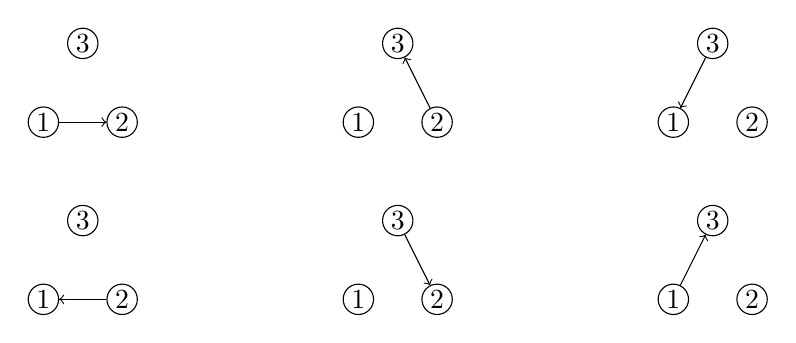
\begin{tikzpicture}
% Set top left
\draw (-4,+2.25) node(n11)[circle,draw=black,inner sep=1pt] {$1$} +(1,0) node(n12)[circle,draw=black,inner sep=1pt] {$2$} +(0.5,1) node(n13)[circle,draw=black,inner sep=1pt] {$3$};
% Set top middle
\draw (+0,+2.25) node(n21)[circle,draw=black,inner sep=1pt] {$1$} +(1,0) node(n22)[circle,draw=black,inner sep=1pt] {$2$} +(0.5,1) node(n23)[circle,draw=black,inner sep=1pt] {$3$};
% Set top right
\draw (+4,+2.25) node(n31)[circle,draw=black,inner sep=1pt] {$1$} +(1,0) node(n32)[circle,draw=black,inner sep=1pt] {$2$} +(0.5,1) node(n33)[circle,draw=black,inner sep=1pt] {$3$};
% Set bottom left
\draw (-4,+0) node(n41)[circle,draw=black,inner sep=1pt] {$1$} +(1,0) node(n42)[circle,draw=black,inner sep=1pt] {$2$} +(0.5,1) node(n43)[circle,draw=black,inner sep=1pt] {$3$};
% Set bottom middle
\draw (+0,+0) node(n51)[circle,draw=black,inner sep=1pt] {$1$} +(1,0) node(n52)[circle,draw=black,inner sep=1pt] {$2$} +(0.5,1) node(n53)[circle,draw=black,inner sep=1pt] {$3$};
% Set bottom right
\draw (+4,+0) node(n61)[circle,draw=black,inner sep=1pt] {$1$} +(1,0) node(n62)[circle,draw=black,inner sep=1pt] {$2$} +(0.5,1) node(n63)[circle,draw=black,inner sep=1pt] {$3$};
% Arrows set 1
\draw[->] (n11) -- (n12);
% Arrows set 2
\draw[->] (n22) -- (n23);
% Arrows set 3
\draw[->] (n33) -- (n31);
% Arrows set 4
\draw[->] (n42) -- (n41);
% Arrows set 5
\draw[->] (n53) -- (n52);
% Arrows set 6
\draw[->] (n61) -- (n63);
\end{tikzpicture}
\caption{Ordered subsets representing the Lah number with $n=3$ and $k=2$.}
\label{figA.3}
\end{figure}

\section{Relations Between the Stirling and Lah Numbers}

The three different combinatorial numbers presented within the previous sections of this appendix are related. It can be seen that they represent a change in basis for polynomial functions as it is pictured by Figure \ref{figA.4}. A Polynomial function can be expressed uniquely with the canonical polynomial basis or with the polynomial basis generated from the rising and the falling factorials. The Figure \ref{figA.4} presents how these numbers connect the three polynomial basis mentioned previously. Therefore, it means that the Stirling number of the first and second kind can be considered as inverses when they form lower triangular matrices whose entries are the Stirling numbers with corresponding row and column indexes. Similarly, as it can be seen Figure \ref{figA.4}, the Lah numbers and the Lah numbers multiplied by $(-1)^{n-k}$ can be seen as inverses when they compose the entries of lower triangular matrices. Finally, since these three combinatorial numbers represent different ways to partition a set of $n$ elements into $k$ subsets being respectively unordered, cyclically ordered and linearly ordered, the following inequalities naturally arise,

\begin{equation} \label{eqnA.14}
\forall (n,k) \in \mathbb{N} \times \mathbb{N} ,\, \genfrac{\{}{\}}{0pt}{0}{n}{k} \leq \genfrac{[}{]}{0pt}{0}{n}{k} \leq \genfrac{\lfloor}{\rfloor}{0pt}{0}{n}{k}
\end{equation}

\begin{figure}[!htbp]
\centering
\begin{tikzpicture}
% Nodes basis
\node (n1) at (0,5) {$x^{n}$};
\node (n2) at (-3,0) {$x^{(n)}$};
\node (n3) at (3,0) {$(x)_{n}$};
% Arrows
\draw[->] (n1) -- node[anchor=north east]{$\genfrac{\{}{\}}{0pt}{0}{n}{k}$} (n3);
\draw (n3) edge[bend right,->] node[anchor=south west]{$(-1)^{n-k}\genfrac{[}{]}{0pt}{0}{n}{k}$} (n1);
\draw[->] (n3) -- node[anchor=south]{$\genfrac{\lfloor}{\rfloor}{0pt}{0}{n}{k}$} (n2);
\draw (n2) edge[bend right,->] node[anchor=north]{$(-1)^{n-k}\genfrac{\lfloor}{\rfloor}{0pt}{0}{n}{k}$} (n3);
\draw[->] (n2) -- node[anchor=north west]{$\genfrac{[}{]}{0pt}{0}{n}{k}$} (n1);
\draw (n1) edge[bend right,->] node[anchor=south east]{$(-1)^{n-k}\genfrac{\{}{\}}{0pt}{0}{n}{k}$} (n2);
\end{tikzpicture}
\caption{Relations between the Stirling and Lah numbers.}
\label{figA.4}
\end{figure} % Appendix 1
%%*******************************************************************************
%********************************* Appendix B **********************************
%*******************************************************************************
\chapter{Graph Theory}
\chaptermark{Graph Theory}
\label{AppendixB}

\section{Introduction}

Multiple real life situations can be modelled by a set of vertices connected together by edges, this representation is called a graph. Graph theory is a field of discrete mathematics that has been developed in order to provide the tools to analyse and solve problems involving graphs, subsequently providing answers to the real life situations they represent \citep{Diestel2000,Bondy2008}. Graphs can be undirected, directed, and even weighted based on the type of situation that is modelled. A given graph $\mathcal{G}$ is defined by an ordered pair of elements, including a set of vertices $V$ and a set of edges $E$ such that, 

\begin{equation} \label{eqnB.1}
\mathcal{G} = (V,E).
\end{equation}

The set of edges $E$ is composed of pairs of vertices taken from the set $V$ that can be directed and even weighted in some cases. Graphs can also be defined by their incidence or adjacency matrices. The incidence matrix of an undirected graph is a rectangle matrix whose rows represent the vertices and whose columns represent the edges, its entries are positive integers representing the number of times a vertex and an edge are incident. The adjacency matrix is a square matrix with rows and columns labelled after the vertices and composed of binaries. When an entry is equal to $1$, it indicates the presence of an edge between the vertices corresponding to the row and column indexes, whereas a $0$ entry  means that there is no direct link between these two particular vertices. A graph is said to be disconnected if its vertices can be partitioned into two distinct subsets that do not share any edges, otherwise a graph is said to be connected.

\section{Undirected Graphs}

An undirected graph also called simple graph is a graph where the edges are not oriented, therefore, the edge $\{1,2\}$ is the same as the edge $\{2,1\}$. A direct consequence of this is that for an undirected graph with $n$ vertices the maximum number of edges is $\frac{n(n-1)}{2}$ if loops are not considered and $\frac{n(n+1)}{2}$ with loops. Two vertices linked by an edge are said to be adjacent, and a vertex is said to be incident with an edge and vice versa. Subsequently, a graph can be defined by its incidence matrix or adjacency matrix. The adjacency matrix of a simple graph is a symmetric binary matrix, the Figure \ref{figB.1} represents a simple undirected graph with $10$ vertices.

\begin{figure}[!htbp]
\centering
\begin{tikzpicture}[scale=4,
	vertex/.style={draw,circle,minimum size=0.75cm,inner sep=0pt},
	arc/.style={draw=blue!#10,thick,->},
	arc label/.style={fill=white,circle,font=\tiny,inner sep=1pt},
	loop arc/.style={min distance=2mm,looseness=8}]
	\foreach [count=\i] \coord in
							{(1.000,0.000),
							 (0.809,0.588),
							 (0.309,0.951),
							 (-0.309,0.951),
							 (-0.809,0.588),
							 (-1.000,0.000),
							 (-0.809,-0.588),
							 (-0.309,-0.951),
							 (0.309,-0.951),
							 (0.809,-0.588)}
							 {
				\node[vertex] (p\i) at \coord {\i};
		}
		\graphfromadj[bend left=0]{p}{{0,0,0,0,10,0,0,0,0,10},
										{10,0,0,0,0,10,0,0,0,0},
										{0,10,0,0,0,0,10,0,0,0},
										{0,0,10,0,0,0,0,10,0,0},
										{0,0,0,10,0,0,0,0,10,0},
										{0,0,0,0,10,0,0,0,0,10},
										{10,0,0,0,0,10,0,0,0,0},
										{0,10,0,0,0,0,10,0,0,0},
										{0,0,10,0,0,0,0,10,0,0},
										{0,0,0,10,0,0,0,0,10,0}}{36}{30}{1}
\end{tikzpicture}
\caption{Example of an undirected graph.}
\label{figB.1}
\end{figure}

The adjacency matrix representation is not unique and any permutations of a row and a column with equal indexes will yield the same graph by changing the vertex labels. A possible adjacency matrix $\mathcal{A}$ for the graph presented in Figure \ref{figB.1} is as follows,

\begin{equation} \label{eqnB.2}
\mathcal{A}=
\begin{bmatrix}
0 & 1 & 0 & 0 & 1 & 0 & 1 & 0 & 0 & 1 \\
1 & 0 & 1 & 0 & 0 & 1 & 0 & 1 & 0 & 0 \\
0 & 1 & 0 & 1 & 0 & 0 & 1 & 0 & 1 & 0 \\
0 & 0 & 1 & 0 & 1 & 0 & 0 & 1 & 0 & 1 \\
1 & 0 & 0 & 1 & 0 & 1 & 0 & 0 & 1 & 0 \\
0 & 1 & 0 & 0 & 1 & 0 & 1 & 0 & 0 & 1 \\
1 & 0 & 1 & 0 & 0 & 1 & 0 & 1 & 0 & 0 \\
0 & 1 & 0 & 1 & 0 & 0 & 1 & 0 & 1 & 0 \\
0 & 0 & 1 & 0 & 1 & 0 & 0 & 1 & 0 & 1 \\
1 & 0 & 0 & 1 & 0 & 1 & 0 & 0 & 1 & 0
\end{bmatrix}
\end{equation}

Similarly, a graph can be defined by its incidence matrix $\mathcal{I}$. This kind of matrix links each edge to the two vertices it connects. The incidence matrix of the graph \ref{eqnB.1} is presented in equation \eqref{eqnB.3}. It can be noted that the adjacency matrix does not have to be symmetric or even square since the number of edges can be different from the number of vertices. In the same way as for the adjacency matrix, any permutations of the rows and the columns will represent the same graph after changing the labels of the vertices and of the edges respectively. Very often graphs have a lot more edges than vertices, subsequently in most cases the adjacency matrix constitutes a more compact way to store a graph than the incidence matrix. Hence, it is the preferred representation in most cases.

\begin{equation} \label{eqnB.3}
\mathcal{I}^{\top}=
\begin{bmatrix}
1 & 1 & 0 & 0 & 0 & 0 & 0 & 0 & 0 & 0 \\
0 & 1 & 1 & 0 & 0 & 0 & 0 & 0 & 0 & 0 \\
0 & 0 & 1 & 1 & 0 & 0 & 0 & 0 & 0 & 0 \\
0 & 0 & 0 & 1 & 1 & 0 & 0 & 0 & 0 & 0 \\
0 & 0 & 0 & 0 & 1 & 1 & 0 & 0 & 0 & 0 \\
0 & 0 & 0 & 0 & 0 & 1 & 1 & 0 & 0 & 0 \\
0 & 0 & 0 & 0 & 0 & 0 & 1 & 1 & 0 & 0 \\
0 & 0 & 0 & 0 & 0 & 0 & 0 & 1 & 1 & 0 \\
0 & 0 & 0 & 0 & 0 & 0 & 0 & 0 & 1 & 1 \\
1 & 0 & 0 & 0 & 0 & 0 & 0 & 0 & 0 & 1 \\
1 & 0 & 0 & 0 & 1 & 0 & 0 & 0 & 0 & 0 \\
1 & 0 & 0 & 0 & 0 & 0 & 1 & 0 & 0 & 0 \\
0 & 1 & 0 & 0 & 0 & 1 & 0 & 0 & 0 & 0 \\
0 & 1 & 0 & 0 & 0 & 0 & 0 & 1 & 0 & 0 \\
0 & 0 & 1 & 0 & 0 & 0 & 1 & 0 & 0 & 0 \\
0 & 0 & 1 & 0 & 0 & 0 & 0 & 0 & 1 & 0 \\
0 & 0 & 0 & 1 & 0 & 0 & 0 & 1 & 0 & 0 \\
0 & 0 & 0 & 1 & 0 & 0 & 0 & 0 & 0 & 1 \\
0 & 0 & 0 & 0 & 1 & 0 & 0 & 0 & 1 & 0 \\
0 & 0 & 0 & 0 & 0 & 1 & 0 & 0 & 0 & 1
\end{bmatrix}
\end{equation}

Graphs are mathematical objects used to represent a given topology and consequently, the relative position of the vertices as well as the shape of the edges does not change the topological properties of a given graph. However, only plotting the undirected edges between a set of vertices can be insufficient sometimes, and in some cases associating an edge with a specific direction can carry some useful meaning. This property is achieved for the directed graphs and presented within the next section.

\section{Directed Graphs}

Each edge of a simple graph can be oriented from a vertex towards another in order to define a directed graph. An edge is called a loop if it connects a vertex to itself. A directed graph also called a digraph does not usually include any loops or parallel edges (multiple edges from and to the same vertex). The graph presented in Figure \ref{figB.2} corresponds to the oriented adjacency matrix $\mathcal{A}$ given equation \eqref{eqnB.4}. In this case the adjacency matrix is still square and composed of binaries entries but does not have to be symmetric any more. Indeed, the adjacency matrix of a digraph contains the information related to the incidence of the edges as well as their orientation. Any element of $\mathcal{A}$ indicates the number of edges starting from the vertex indexed by the row index and going to the vertex indexed by the column index. Directed graphs do not only inform on the topology but also on the direction of the edges between the vertices, therefore, they can be used to represent a succession of states or flows between vertices. In the example presented Figure \ref{eqnB.2}, each vertex is the initial vertex of two edges and the terminal vertex of two other edges.

\begin{figure}[!htbp]
\centering
\begin{tikzpicture}[scale=4,
		vertex/.style={draw,circle,minimum size=0.75cm,inner sep=0pt},
		arc/.style={draw=blue!#10,thick,->},
		arc label/.style={fill=white,circle,font=\tiny,inner sep=1pt},
		loop arc/.style={min distance=2mm,looseness=8}
		]
		\foreach [count=\i] \coord in
							{(1.000,0.000),
							 (0.809,0.588),
							 (0.309,0.951),
							 (-0.309,0.951),
							 (-0.809,0.588),
							 (-1.000,0.000),
							 (-0.809,-0.588),
							 (-0.309,-0.951),
							 (0.309,-0.951),
							 (0.809,-0.588)}
							 {
				\node[vertex] (p\i) at \coord {\i};
		}
		\directedgraphfromadj[bend left=5]{p}{{0,0,0,0,0,0,10,0,0,10},
											{10,0,0,0,0,0,0,10,0,0},
											{0,10,0,0,0,0,0,0,10,0},
											{0,0,10,0,0,0,0,0,0,10},
											{10,0,0,10,0,0,0,0,0,0},
											{0,10,0,0,10,0,0,0,0,0},
											{0,0,10,0,0,10,0,0,0,0},
											{0,0,0,10,0,0,10,0,0,0},
											{0,0,0,0,10,0,0,10,0,0},
											{0,0,0,0,0,10,0,0,10,0}}{36}{30}{1}
\end{tikzpicture}
\caption{Example of a directed graph.}
\label{figB.2}
\end{figure}

Consequently, in this specific case the binary entries of the adjacency matrix $\mathcal{A}$ are positioned in such a way that each row and each column sum to two. A row sums to two for two edges leaving a vertex and a column sums to two for two edges going to a vertex.

\begin{equation} \label{eqnB.4}
\mathcal{A}=
\begin{bmatrix}
0 & 0 & 0 & 0 & 0 & 0 & 1 & 0 & 0 & 1 \\
1 & 0 & 0 & 0 & 0 & 0 & 0 & 1 & 0 & 0 \\
0 & 1 & 0 & 0 & 0 & 0 & 0 & 0 & 1 & 0 \\
0 & 0 & 1 & 0 & 0 & 0 & 0 & 0 & 0 & 1 \\
1 & 0 & 0 & 1 & 0 & 0 & 0 & 0 & 0 & 0 \\
0 & 1 & 0 & 0 & 1 & 0 & 0 & 0 & 0 & 0 \\
0 & 0 & 1 & 0 & 0 & 1 & 0 & 0 & 0 & 0 \\
0 & 0 & 0 & 1 & 0 & 0 & 1 & 0 & 0 & 0 \\
0 & 0 & 0 & 0 & 1 & 0 & 0 & 1 & 0 & 0 \\
0 & 0 & 0 & 0 & 0 & 1 & 0 & 0 & 1 & 0
\end{bmatrix}
\end{equation}

The representation of a directed graph by its incidence matrix is done by adding signs to the matrix entries. An entry is set to $-1$ if an edge leaves a vertex and to $1$ if an edge points towards a vertex, it is set to $0$ otherwise.

\section{Weighted Graphs}

In some cases it is important to associate each oriented edge of a directed graph to a weight. Weighted graphs are used to define a certain distance closeness between two given vertices and are therefore essential to analyse the flow between vertices. In the same way as for the simple graphs and the directed graphs, weighted graphs could be defined by their incidence or adjacency matrix.

\begin{figure}[!htbp]
\centering
\begin{tikzpicture}[scale=4,
		vertex/.style={draw,circle,minimum size=0.75cm,inner sep=0pt},
		arc/.style={draw=blue!#10,thick,->},
		arc label/.style={fill=white,circle,font=\tiny,inner sep=1pt},
		loop arc/.style={min distance=2mm}
		]
		\foreach [count=\i] \coord in
							{(1.000,0.000),
							 (0.809,0.588),
							 (0.309,0.951),
							 (-0.309,0.951),
							 (-0.809,0.588),
							 (-1.000,0.000),
							 (-0.809,-0.588),
							 (-0.309,-0.951),
							 (0.309,-0.951),
							 (0.809,-0.588)}
							 {
				\node[vertex] (p\i) at \coord {\i};
		}
		\weigthedgraphfromadj[bend left=10]{p}{{0,0,0,0,0,0,5,0,0,9},
												 {2,0,0,0,0,0,0,2,0,0},
												 {0,5,0,0,0,0,0,0,5,0},
												 {0,0,7,0,0,0,0,0,0,10},
												 {7,0,0,9,0,0,0,0,0,0},
												 {0,6,0,0,2,0,0,0,0,0},
												 {0,0,5,0,0,1,0,0,0,0},
												 {0,0,0,5,0,0,2,0,0,0},
												 {0,0,0,0,8,0,0,5,0,0},
												 {0,0,0,0,0,3,0,0,8,0}}{36}{30}{1}
\end{tikzpicture}
\caption{Example of a weighted graph.}
\label{figB.3}
\end{figure}

The adjacency matrix of a weighted graph has to contain the necessary information about the weights and the orientations of all the edges. A weight is located on the entry at the intersection of the row and the column, whose indexes are the index of the initial vertex and of the terminal vertex respectively. The entries of the incidence matrix are the weights of the edges with positive and negative signs, positive for an edge that is directed from a vertex and negative for an edge directed towards a vertex.

\section{Multi-graphs}

Finally, multi-graphs allow to have multiple weighted edges between two given vertices, also a given vertex can be connected to itself by a loop. Therefore, multi-graphs subsume the oriented and weighted graphs into one single type of graph. In the same way as before they can be represented by an adjacency matrix $\mathcal{A}$ as presented equation \eqref{eqnB.5} or by an incidence matrix. The multi-graph linked to the adjacency matrix $\mathcal{A}$ is shown in Figure \ref{figB.4}. The adjacency matrix contains the orientation of each edge as well as their respective weights, subsequently it is a square matrix linking the vertices with weights. The edges connect the vertices indexed by the row indexes to the ones indexed by the column indexes with the weight provided by the value of the matrix entry. The incidence matrix has the same definition as the incidence matrix for the weighted graphs, possibly including many parallel edges as well as loops.

\begin{equation} \label{eqnB.5}
\mathcal{A}=
\begin{bmatrix}
1 & 5 & 0 & 0 & 1 & 0 & 5 & 0 & 0 & 5 \\
2 & 2 & 1 & 0 & 0 & 5 & 0 & 2 & 0 & 0 \\
0 & 5 & 3 & 2 & 0 & 0 & 2 & 0 & 5 & 0 \\
0 & 0 & 7 & 4 & 5 & 0 & 0 & 2 & 0 & 5 \\
7 & 0 & 0 & 7 & 5 & 5 & 0 & 0 & 1 & 0 \\
0 & 5 & 0 & 0 & 2 & 6 & 5 & 0 & 0 & 1 \\
2 & 0 & 5 & 0 & 0 & 1 & 7 & 5 & 0 & 0 \\
0 & 7 & 0 & 5 & 0 & 0 & 2 & 8 & 1 & 0 \\
0 & 0 & 5 & 0 & 7 & 0 & 0 & 5 & 9 & 1 \\
5 & 0 & 0 & 5 & 0 & 1 & 0 & 0 & 1 & 10
\end{bmatrix}
\end{equation}

\begin{figure}[!htbp]
\centering
\begin{tikzpicture}[scale=4,
		vertex/.style={draw,circle,minimum size=0.75cm,inner sep=0pt},
		arc/.style={draw=blue!#10,thick,->},
		arc label/.style={fill=white,circle,font=\tiny,inner sep=1pt},
		loop arc/.style={loop,min distance=2mm}
		]
		\foreach [count=\i] \coord in
							{(1.000,0.000),
							 (0.809,0.588),
							 (0.309,0.951),
							 (-0.309,0.951),
							 (-0.809,0.588),
							 (-1.000,0.000),
							 (-0.809,-0.588),
							 (-0.309,-0.951),
							 (0.309,-0.951),
							 (0.809,-0.588)}
							 {
				\node[vertex] (p\i) at \coord {\i};
		}
		\weigthedgraphfromadj[bend left=10]{p}{{1,5,0,0,1,0,5,0,0,5},
											 {2,2,1,0,0,5,0,2,0,0},
											 {0,5,3,2,0,0,2,0,5,0},
											 {0,0,7,4,5,0,0,2,0,5},
											 {7,0,0,7,5,5,0,0,1,0},
											 {0,5,0,0,2,6,5,0,0,1},
											 {2,0,5,0,0,1,7,5,0,0},
											 {0,7,0,5,0,0,2,8,1,0},
											 {0,0,5,0,7,0,0,5,9,1},
											 {5,0,0,5,0,1,0,0,1,10}}{36}{30}{1}
\end{tikzpicture}
\caption{Example of a weighted multi-graph.}
\label{figB.4}
\end{figure} % Appendix 2

\backmatter
%*******************************************************************************
%********************************* Bibliography ********************************
%*******************************************************************************
%\nocite{*}
\bibliographystyle{Bibliography/ifac.bst}
\bibliography{Bibliography/libraryOut}

\end{document}